The model is calibrated to Sri Lanka before 2007, when the Chinese government started to provide the increasing amount of loans (see \autoref{fig: sri-lanka-debt-ts}).
\begin{figure}[t]
    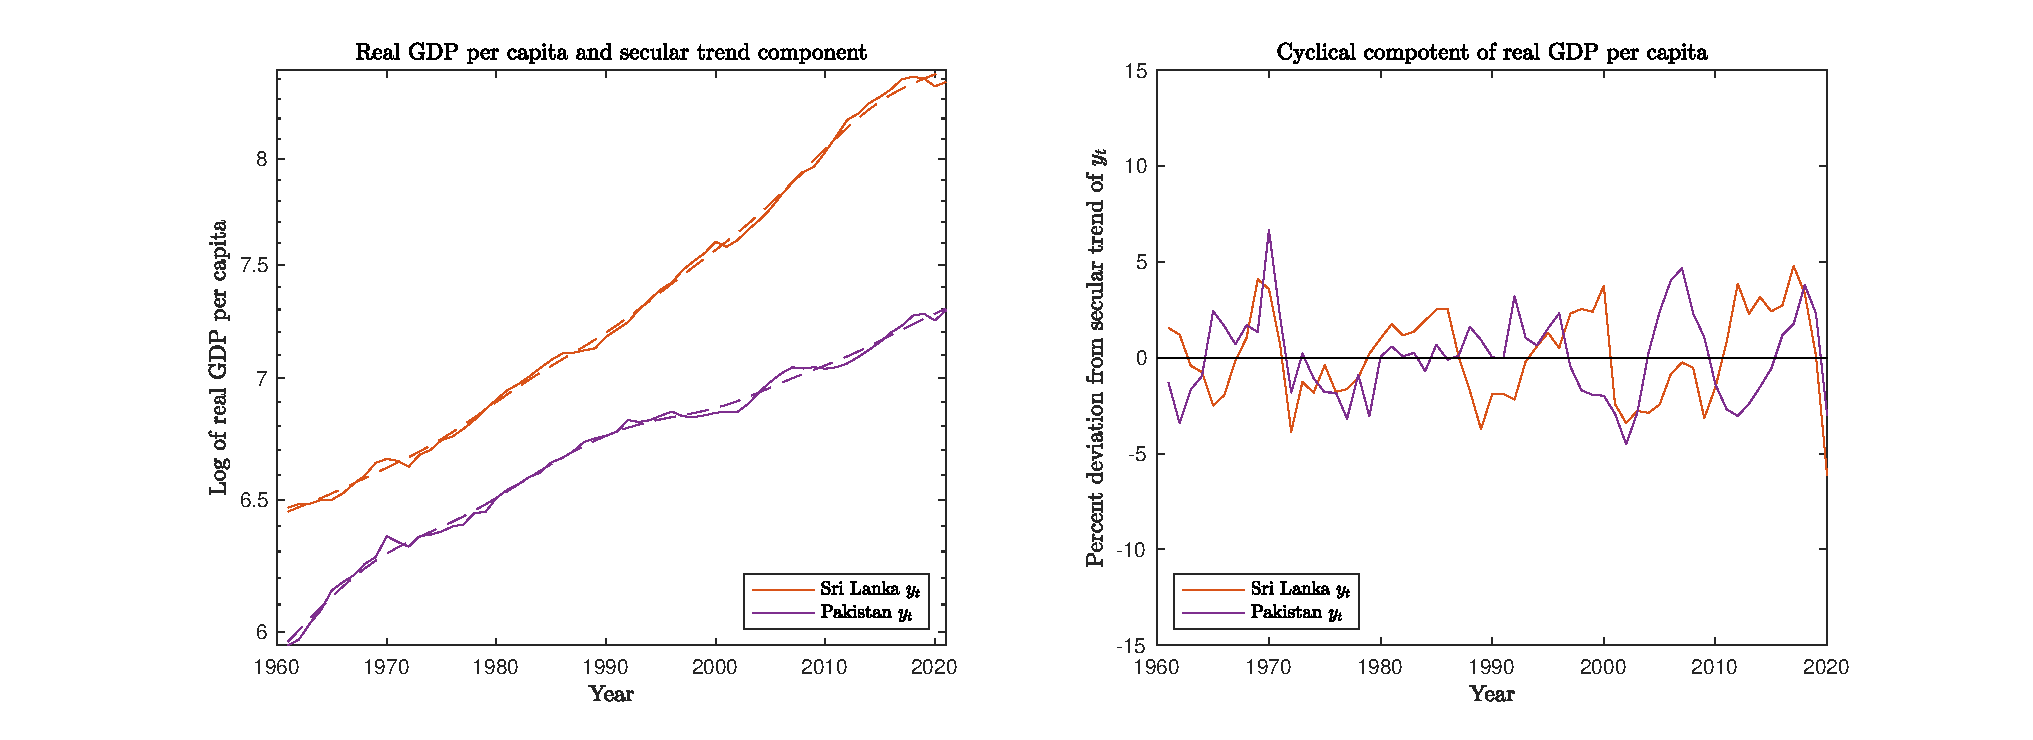
\includegraphics[width = \textwidth]{fig/decompose_gdp.eps}
    \caption{Decomposition of log-real-tradable-GDP for Sri Lanka and Pakistan}
    \label{fig:decompose-gdp}
    \floatfoot{\emph{Source:} World Bank national accounts data. \\
    \emph{Note:} The cyclical component in the right is obtained by the HP-filter with smoothing parameter $\lambda = 100$ for the log-real-GDP in the left. The quarterized AR(1) estimation for Sri Lanka yields $(\rho, \sigma_u)= (0.9114, 0.0123)$, and for Pakistan yields $(\rho, \sigma_u)= (0.9008, 0.0111)$}
\end{figure}

I proxy the output process of \refeq{eq:ar1-output} by the detrended log-real-GDP of Sri Lanka from 1980 to 2021. Considering that the seasonality in the quarterly data for Sri Lanka might impose a higher volatility estimated in the AR(1) process, I follow \citet{Hinrichsen_2020-chapter4} and estimate the annual data over 1980 to 2021. I obtain the cyclical component of the output by filtering the time series with an HP-filter with smoothing parameter $\lambda$ set to 100.
Estimation of the AR(1) on the cyclical component thus yields $\rho = $ 0.9114 and $\sigma_u = $ 0.0123\footnotemark{}. \autoref{fig:decompose-gdp} presents the decomposition of the log-real-GDP.
\footnotetext{Since the AR(1) estimation is conducted on annual data, the estimated coefficients must be quarterized. Specifically,
$\rho = 1 - \frac{1 - \hat{\rho}}{4}$, and $\sigma_u = \frac{\hat{\sigma}}{\sqrt{4}}$, where $\hat{\rho}$ and $\hat{\sigma}$ are the estimated parameters for the AR(1) via OLS.}

The global risk-free world interest rate $r^*$ is set to match the 3-month treasury bill rate during the period, which is roughly 4\% annually, or 1\% for one quarter. This is in line with \citet{Chatterjee-12}.
The probability of reentry is difficult to assess since Sri Lanka encountered its first default in April 12, 2022, and is not yet undergoing the process of restructuring. As a result, following \citet*{Chatterjee-12} and \citet*{Hinrichsen_2020-chapter4}, I set the probability of reentry to 0.0385, which implies that the country will be in default on average for about 6.5 years, matching the median of time spans for past 100 systemic crises \citep*{Reinhart-Rogoff-2014-100-episode}.

Calibration on other structural parameters regarding the Sri Lanka economy follows \citet*{Jegajeevan-Sri-Lanka-DSGE}. The author estimates the Sri Lanka economy with a DSGE model, and based on her calibration, the share of labor is set as 65\%. As the author adopts a CES aggregator for the home and foreign consumption as well, I directly refer to her estimation; that gives $a =$ 0.35 and $\xi=$ 0.78\footnotemark{}.
\footnotetext{\citet*{Jegajeevan-Sri-Lanka-DSGE} calibrates the share of foreign goods (tradable goods) based on the average expenditure on imported goods of 35\% according to the consumer price index. The elasticity of substitution between tradable and nontradable goods is obtained via the posterior mean of the Bayesian estimation within 2008 to 2014.}
This implies that $\sigma = 1/\xi = $ 1.28.

% Please add the following required packages to your document preamble:
% \usepackage{booktabs}
% \usepackage{graphicx}
\begin{table}[h]
    \centering
    % \footnotesize
    \begin{tabular}{@{}llll@{}}
    % \begin{tabular}{@{}lp{0.6\textwidth}lp{0.3\textwidth}@{}}
        \toprule
    Parameter  & Description                                                       & Value  & Source                                                                         \\ \midrule
    $\rho$     & Autocorrelation of output                                         & 0.9114  & Estimation of AR(1) on GDP\\
    $\sigma_u$ & Standard deviation of output                                      & 0.0123 & Estimation of AR(1) on GDP \\
    $r^*$      & Risk-free rate                                                    & 0.01 & U.S. 3-month treasury bill rate \\
    $\theta$   & Probability of reentry                                            & 0.0385 & \citet*{Chatterjee-12}                                              \\
    $\alpha$   & Labor share in non-tradable goods sector                          & 0.65   & \citet{Jegajeevan-Sri-Lanka-DSGE}                                                       \\
    $a$        & Share of tradable consumption                                     & 0.35   & Share of tradable goods in GPD                  \\
    $\xi$      & Intratemporal elasticity of substitution of consumption & 0.5   & \citet{Na-18}                             \\
    $\sigma$   & Inverse of intertemperal elasticity of substitution of consumption  & 2   & $1 / \xi$                                                                      \\
    $\beta$    & Discount factor                                                   & (\dots)  &  Self-estimated                                                                              \\
    $\delta_1$ & Coefficient of the linear term in loss function                   &  (\dots) &   Self-estimated                                                                             \\
    $\delta_2$ & Coefficient of the quadratic term in loss function                &  (\dots)   &               Self-estimated                                                                 \\
    $\bar{h}$  & Labor endowment                                                   & 1      & Normalized to 1\\
    \bottomrule
    \end{tabular}%
    \caption{Calibration for Sri Lanka}
    \label{tab:cal-sri-lanka}
    \floatfoot{\emph{Note}: The time unit is one quarter. AR(1) is performed on annual tradable GDP data but quarterized following the approach of \citet*{Hinrichsen_2020-chapter4}. }
    \end{table}
Following \citet{Na-18}, the rest of the parameters $\left( \beta, \delta_1, \delta_2 \right)$, which is respectively the subjective discount factor and the two parameter for the loss function, is chosen to match three equilibrium outcomes\footnote{
    In particular, I use the grid search algorithm to search for the optimal values for the three parameters. Essentially, VFI must be proceeded for each triplet of the parameters to obtain the targeting equilibrium outcomes. Details are mentioned in \autoref{sec:computation}.
}:
\begin{enumerate*}[label = (\roman*)]
    \item the average debt-to-GDP ratio in periods of good standing is 84\% per quarter;
    \item the frequency of default is 1.37 times per century; and
    \item the average output loss is 10.5\% per year conditional on being in financial autarky.
\end{enumerate*}
The average debt-to-GDP ratio to be targeted is motivated by the fact that the average annual debt-to-GDP ratio in the data is about 42\%\footnotemark{}.
\footnotetext{Data source: International Debt Statistics. The value is calculated by averaging the nominal debt-to-GDP ratio over 2000 to 2010. The same approach is conducted when calibrating Pakistan. }
Multiplying this by an average of 50\% haircut implies that about 21\% of the debt is secured annually\footnotemark{}.
\footnotetext{In the mode, we assume that the country defaults on 100\% of the debt, hence this approach is necessary to handle the case of a haircut.}
Since we are dealing with a model with quarterly period, this results in the 84\% debt-to-GDP ratio.
The average frequency of default is justified by the fact that Sri Lanka experienced its first default on 2022 since its independence in 1948; this give an average of 1.37 times per century\footnote{$\frac{1}{2022-1948} \times 100 \approx 1.37$}. Finally, following the default of Sri Lanka since April 2022, the GDP growth is -7.4\%, -11.5\%, and -12.4\%, for the subsequent three quarters\footnote{Data Source: Central Bank of Sri Lanka}. This implies a geometric mean of -10.5\%.
Table \ref{tab:cal-sri-lanka} summarizes the calibrated parameters and their sources.

